\documentclass{report}
\usepackage[margin=1in, paperwidth=8.5in, paperheight=11in]{geometry}
%Math packages%
\usepackage{amsmath}
\usepackage{amsthm}
%Spacing%
\usepackage{setspace}
\onehalfspacing
%Lecture number%
\newcommand{\lectureNum}{15}
%Variables - Date and Course%
\newcommand{\curDate}{February 28, 2017}
\newcommand{\course}{CS 241}
\newcommand{\instructor}{Kevin Lanctot}
%Defining the example tag%
%\theoremstyle{definition}%
\newtheorem{ex}{Example}[section]
%Setting counter given the lecture number%
\setcounter{chapter}{\lectureNum{}}
%Package to insert code%
\usepackage{listings}
\usepackage{courier}
\usepackage{xcolor}
\lstset { %
    tabsize=2,
    breaklines=true,
    language=C++,
    backgroundcolor=\color{blue!8}, % set backgroundcolor
    basicstyle=\footnotesize\ttfamily,% basic font setting
}
%Package for images%
\usepackage{graphicx}

\begin{document}
%Note title%
\begin{center}
\begin{Large}
\textsc{\course{} | Lecture \lectureNum{}}
\end{Large}
\end{center} 
\noindent \textit{Bartosz Antczak} \hfill
\textit{Instructor: \instructor{}} \hfill
\textit{\curDate{}}
\rule{\textwidth}{0.4pt}
% Actual Notes%
\section{Bottom-up Parsing}
Our old strategy was using a leftmost derivation, called ``LL" parsing. Now we will look at \textit{LR Parsing}, which is more powerful than LL parsing. Basically, LR parsing does what LL parsing does, except backwards.
\subsubsection{Working with the Stack in LR Parsing}
To start, keep on shifting input onto the stack until you have a match with the right hand side of some production rule. If you match with some production rule, then you reduce your stack by changing the right hand side of some production rule to the left hand side.\\
From this, a natural question arises:
\begin{center}
\textit{How do you know when to shift and when to reduce?}
\end{center}
We introduce a place holder ``*" to help us keep track of where we are in the RHS of a production rule, for instance:
\begin{figure}[ht]
\begin{center}
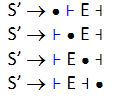
\includegraphics[scale=0.9]{lr1.jpg}
\end{center}
\caption{Here, the place holder is depicted as a black dot. Courtesy of Prof. Lanctot's slides.}
\end{figure}
This allows us to keep track of the place holder.
%END%
\end{document}